\documentclass[14pt]{beamer}

\usetheme{Madrid}

% Add frame numbers
\setbeamertemplate{page number in head/foot}[framenumber]

\usepackage{amsmath, amssymb}
\usepackage{tikz}
\usepackage{bm}
\usepackage{outlines}   % For multilevel lists using the outline environment


\newcommand{\CMA}{Causal Mediation Analysis}
\newcommand{\bE}{\mathbb{E}}
\newcommand{\GLMMs}{Mixed-Effects Models}

\title[]{Statistical Considerations in Multilevel Mediation Analysis}
\author{William Ruth}
\institute[]{Collaborators: Rado Ramasy, Rowin Alfaro, Ariel Mundo, Bruno Remillard, Bouchra Nasri}
\date{\vspace{-3cm}}
\titlegraphic{
\includegraphics[width=2cm]{../Logos/CANSSI_Logo.png} \hspace{2cm} 
\includegraphics[width=4cm]{../Logos/Logo_UdeM-CMJN.jpg}}


\begin{document}

\begin{frame}
    \titlepage
\end{frame}

\begin{frame}{Outline}
    \begin{itemize}
        \setlength{\itemsep}{0.75em}
        \item[1)] The Problem
        \item[2)] Mediation Analysis
        \item[3)] Causal Inference
        \item[4)] Mixed-Effects Models
        \item[234)] Mixed-Effects Models in Causal Mediation Analysis
    \end{itemize}
\end{frame}

\begin{frame}{Example}
    \begin{itemize}
        \item Goal: Understand adherence to restrictive measures
        \begin{itemize}
            \item E.g. Lockdowns
            \item Both past and future \newline
        \end{itemize}
        \item Influence of news source
        \begin{itemize}
            \item How trustworthy? \newline
        \end{itemize}
        \item Disentangle influence on future from influence on past
    \end{itemize}
    
\end{frame}


\begin{frame}{Example}
        \begin{figure}[H]
            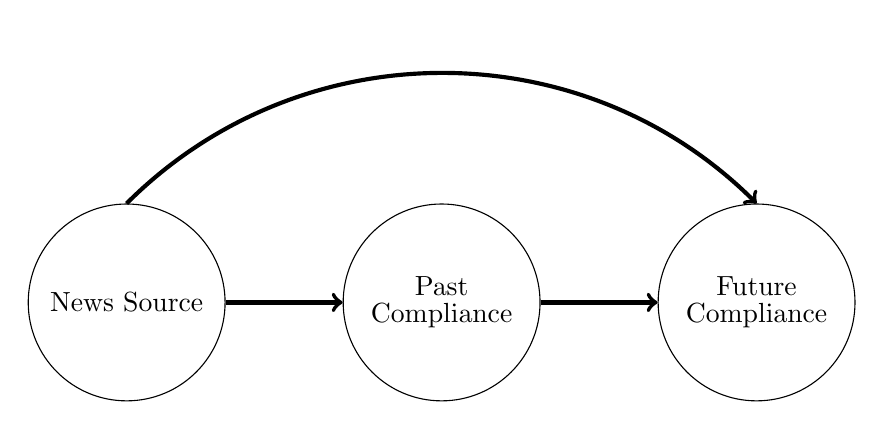
\begin{tikzpicture}
                % Circles with labels
                \node at (0,0) [circle, draw, minimum size=2.5cm] (news) {News Source};
                \node at (4,0) [circle, draw, minimum size=2.5cm] (past) {\shortstack{Past\\Compliance}};
                \node at (8,0) [circle, draw, minimum size=2.5cm] (future) {\shortstack{Future\\Compliance}};
                
                % Arrows
                \draw[->, line width=1.5pt] (news.east) -- (past.west);
                \draw[->, line width=1.5pt] (past.east) -- (future.west);
                \draw[->, line width=1.5pt, bend left] (news.north) to [out=45,in=135] (future.north); 
                
                \end{tikzpicture}
    \end{figure}
\end{frame}

\begin{frame}{Example}
    Terminology
    \begin{columns}
        \column{0.6\textwidth}
        \begin{itemize}
            \item Top path: {Direct effect}
            \item Center path: {Indirect effect}
            \item Combined: {Total effect}
        \end{itemize}
        \column{0.4\textwidth}
        \begin{itemize}
            \item Exposure: $X$
            \item Outcome: $Y$
            \item Mediator: $M$
        \end{itemize}
    \end{columns}
    
\end{frame}




\begin{frame}{Mediation Analysis}
    \begin{figure}[H]
        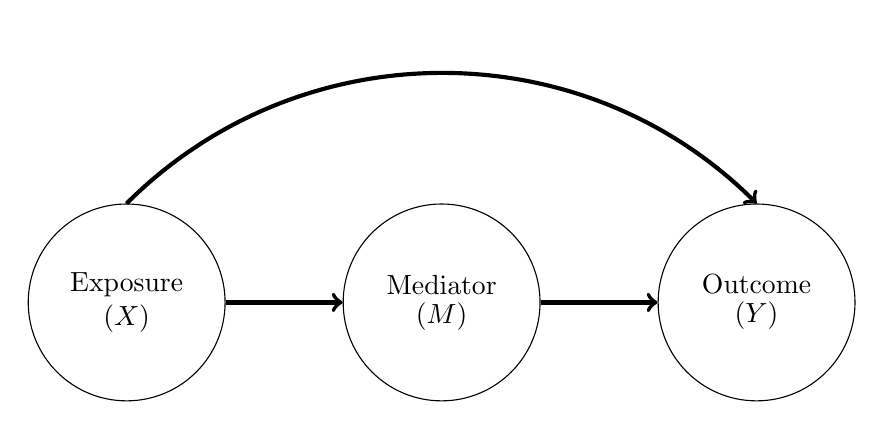
\begin{tikzpicture}
            % Circles with labels
            \node at (0,0) [circle, draw, minimum size=2.5cm] (X) {\shortstack{Exposure\\($X$)}};
            \node at (4,0) [circle, draw, minimum size=2.5cm] (M) {\shortstack{Mediator\\($M$)}};
            \node at (8,0) [circle, draw, minimum size=2.5cm] (Y) {\shortstack{Outcome\\($Y$)}};
            
            % Arrows
            \draw[->, line width=1.5pt] (X.east) -- (M.west);
            \draw[->, line width=1.5pt] (M.east) -- (Y.west);
            \draw[->, line width=1.5pt, bend left] (X.north) to [out=45,in=135] (Y.north); 
            
            \end{tikzpicture}
    \end{figure}
\end{frame}

\begin{frame}{Mediation Analysis}
    Separate \textbf{Total Effect} of $X$ on $Y$ into
    \begin{itemize}
        \item \textbf{Direct Effect}
        \item \textbf{Indirect Effect}\newline
    \end{itemize}

    Traditionally, use regression
\end{frame}

\begin{frame}{Mediation Analysis}
    Continuous outcome and mediator:
    \begin{itemize}
        \item $Y = \alpha_0 + \alpha_1 M + \alpha_2 X + \varepsilon_Y$
        \item $M = \beta_0 + \beta_1 X + \varepsilon_M$ \newline
    \end{itemize}

    
    \textbf{Direct Effect}: $\alpha_2$
    \begin{itemize}
        \item ``$X$ in $Y$''
    \end{itemize}
    \textbf{Indirect Effect}: $\alpha_1 \cdot \beta_1$
    \begin{itemize}
        \item ``$M$ in $Y$'' $\cdot$ ``$X$ in $M$''
    \end{itemize}
    \textbf{Total Effect}: $\alpha_2 + \alpha_1 \cdot \beta_1$

\end{frame}

\begin{frame}{Mediation Analysis}
    Popular approach
    \begin{itemize}
        \item A bit outdated\ldots \newline
    \end{itemize}

    More popular: Causal mediation analysis
    
\end{frame}

\begin{frame}{Causal Inference}
    Assume that $X$ \textit{causes} $Y$\newline

    Counterfactuals:
    \begin{itemize}
        \item What value would $Y$ take if $X$ were set to a particular level?
        \item Write $Y_x$ for the value of $Y$ when $X=x$
        \item If $X\neq x$ then $Y_x$ is literally a ``counterfactual'' 
    \end{itemize}
\end{frame}

\begin{frame}{Causal Inference}
    Example:
    \begin{itemize}
        \item Alice only reads scientific publications and will follow all lockdown mandates
        \item What if she instead only read Facebook?\newline
        \item $Y_{Science}(Alice) = \mathrm{follow}$
        \item $Y_{Facebook}(Alice) = \mathrm{follow}$
    \end{itemize}
\end{frame}

\begin{frame}{Causal Inference}
    Example:
    \begin{itemize}
        \item Bob also only reads scientific publications and will follow all lockdown mandates, but is more susceptible to being influenced \newline
        \item $Y_{Science}(Bob) = \mathrm{follow}$
        \item $Y_{Facebook}(Bob) = \mathrm{not\ follow}$
    \end{itemize}
\end{frame}

\begin{frame}{Causal Inference}
    \begin{itemize}
        \item We only observe one outcome per individual\newline

        \item Explore population-level effects by averaging\newline

        \item Define mediation effects in terms of expected counterfactuals
    \end{itemize}
\end{frame}

\begin{frame}{Causal Inference}
    \textbf{Total Effect}: $\mathbb{E}(Y_{x'} - Y_{x})$
    \begin{itemize}
        \item Effect on outcome when we change exposure from $X=x$ to $X=x'$ \newline
    \end{itemize}

    Other effects involve dependence on a mediator:
    \begin{itemize}
        \item $Y_{xm}$: Value of outcome when
        \begin{itemize}
            \item Exposure ($X$) is set to $x$
            \item Mediator ($M$) is set to $m$
        \end{itemize}
        \item $M_x$: Value of mediator when
        \begin{itemize}
            \item Exposure ($X$) is set to $x$
        \end{itemize}
        \item ``Nested Counterfactuals'': $Y_{x M_x}$ or $Y_{x M_{x'}}$
    \end{itemize}

\end{frame}

\begin{frame}{Causal Mediation Analysis}
    \textbf{Controlled Direct Effect}: $\mathbb{E}(Y_{x'm} - Y_{xm})$
    \begin{itemize}
        \item Effect of changing exposure with mediator held fixed \newline
    \end{itemize}

    \textbf{Natural Direct Effect}: $\mathbb{E}(Y_{x'M_{x}} - Y_{xM_{x}})$
    \begin{itemize}
        \item Effect of changing exposure when we don't interfere with the mediator  \newline
    \end{itemize}

    \textbf{Natural Indirect Effect}: $\mathbb{E}(Y_{xM_{x'}} - Y_{xM_{x}})$
    \begin{itemize}
        \item Effect of changing which exposure value is seen by the mediator while holding fixed which exposure value is seen by the outcome
    \end{itemize}
\end{frame}

\begin{frame}{\CMA}
    In our example
    \begin{itemize}
        \item Controlled Direct Effect: Effect of increasing news trustworthiness if the whole population followed guidelines in the past
        \item Natural Direct Effect: Effect of increasing news trustworthiness independent of any induced change in past compliance
        \item Natural Indirect Effect: Effect of changing past compliance if everyone only got news from Facebook
    \end{itemize}
\end{frame}

\begin{frame}{\CMA}
    We can't measure all required counterfactuals
    \begin{itemize}
        \item E.g., $Y_x$ or $Y_{x'}$, not both \newline
    \end{itemize}

    Expected counterfactuals related to conditional expectations

    \begin{itemize}
        \item     Under strong assumptions, $\bE Y_x = \bE(Y | X=x)$ \newline
    \end{itemize}

    Nested counterfactuals more complicated
    \begin{itemize}
        \item More on this later
    \end{itemize}
\end{frame}

\begin{frame}{\CMA}
    How does causality change our analysis? \newline

    Still fit regression models, but include interaction terms between exposure and mediator
    \begin{itemize}
        \item $Y = \alpha_0 + \alpha_1 M + \alpha_2 X + \alpha_3 M \cdot X + \varepsilon_Y$
        \item $M = \beta_0 + \beta_1 X + \varepsilon_M$ \newline
    \end{itemize}

    Direct and indirect effects now depend on the levels of the exposure

\end{frame}


\begin{frame}{\CMA\ -- Extensions}
    Discussion so far has involved continuous mediator and outcome
    \begin{itemize}
        \item What about binary or categorical? \newline
    \end{itemize}

    Individuals might also be clustered
    \begin{itemize}
        \item E.g. Within countries
    \end{itemize}

\end{frame}

\begin{frame}{\CMA\ -- Extensions}
    Handling binary variables is pretty straightforward
    \begin{outline}
        \1 Instead of linear regression, use logistic regression
        \1 Re-define mediation effects based on expected counterfactuals
            \2 I.e. Counterfactual probabilities
        \1 New formulas for relating mediation effects to regression coefficients \newline
    \end{outline}

    Extend to more than 2 categories using binary indicators
\end{frame}

\begin{frame}{\CMA\ -- Extensions}
    Clustered data more complicated \newline

    Standard approach is multi-level modelling
    \begin{itemize}
        \item I.e. Add random effects that vary across clusters \newline
    \end{itemize}

    Combined with categorical variables: 
    \begin{itemize}
        \item Generalized linear mixed models (GLMMs)
    \end{itemize}
\end{frame}


\begin{frame}{\GLMMs}
    The core idea is to augment our set of covariates
    \begin{itemize}
        \item Coefficients of these new covariates are random variables that vary across groups/clusters \newline
    \end{itemize}

    In the linear setting:
    \begin{itemize}
        \item Old model: \newline
        $Y = \alpha_0 + \alpha_1 X_1 + \ldots + \alpha_p X_p + \varepsilon$
        \item New model:  \newline
        $Y = \alpha_0 + \alpha_1 X_1 + \ldots + \alpha_p X_p$ \newline
        \hspace{1cm} $\mathbf{+ u_1 Z_1 + \ldots + u_q Z_q} + \varepsilon$ 
    \end{itemize}

    


\end{frame}

\begin{frame}{\GLMMs}
    The $Z$'s are fixed, known covariates
    The $u$'s are random variables
    \begin{itemize}
        \item I.e. Random effects \newline
    \end{itemize}

    It's possible for the $X$'s and $Z$'s to overlap
    \begin{itemize}
        \item The coefficient on such a covariate has the form $\alpha_j + u_{k}$
        \item I.e. Mixed effect
    \end{itemize}

\end{frame}


\begin{frame}{\GLMMs}
    Extend to generalized linear models in the usual way \newline

    Choose response distribution and link function as for ordinary GLMs \newline

    Linear predictor now has a random effects component \newline
\end{frame}

\begin{frame}{\GLMMs}
    Why bother?
    \begin{itemize}
        \item E.g. Measured some but not all levels of a categorical variable
        \item Estimate covariance matrix of random effects
        \item Test for non-zero variance of each random effect \newline
    \end{itemize}

    ``Predict'' level of random effects for each group
    \begin{itemize}
        \item Conditional mean or conditional mode of random effects given response
    \end{itemize}
\end{frame}

\begin{frame}{\GLMMs}
    In our example:
    \begin{itemize}
        \item Data collected from 11 different countries
        \item Explicitly model inter-country variability
        \item Predict country-specific random effects
        \item Use country-specific coefficients in formulas for mediation effects
        \item Test for significant mediation effects within each country \newline
    \end{itemize}
\end{frame}

\begin{frame}{Multilevel Mediation Analysis}
    Uncertainty quantification for mixed-effects models can be challenging  \newline
    
    Strategies include:
    \begin{itemize}
        \item Bootstrap
        \item Quasi-Bayesian Monte Carlo
        \item $\delta$-method
    \end{itemize}
\end{frame}

\begin{frame}{Multilevel Mediation Analysis}
    Uncertainty quantification for mixed-effects models can be challenging  \newline
    
    Strategies include:
    \begin{itemize}
        \item \textbf{Bootstrap} (Rado Ramasy, yesterday)
        \item Quasi-Bayesian Monte Carlo
        \item $\delta$-method
    \end{itemize}
\end{frame}

\begin{frame}{Multilevel Mediation Analysis}
    Uncertainty quantification for mixed-effects models can be challenging  \newline
    
    Strategies include:
    \begin{itemize}
        \item Bootstrap
        \item Quasi-Bayesian Monte Carlo
        \item $\bm{\delta}$\textbf{-method}
    \end{itemize}
\end{frame}


\begin{frame}{Multilevel Mediation Analysis}
    Recall: Mediation effects defined using nested counterfactuals -- $ Y_{xM_{x'}}$
    \begin{itemize}
        \item Value of $Y$ when $X$ is set to $x$, and
        \item $M$ is set to whatever value it would have if $X$ were set to $x'$ \newline
    \end{itemize}
    
    Under strong assumptions, use the ``Mediation Formula''
    
\end{frame}

\begin{frame}{Multilevel Mediation Analysis}
    Mediation Formula:
    \begin{align*}
        \action<+->{\bE Y_{xM_{x'}} &= \bE_{M | X=x'} \bE (Y | X=x, M) \\}
    &\action<+->{= \sum_{m=0}^1 \mathbb{P}(Y = 1 | X=x, M=m) \mathbb{P}(M = m | X = x')}
    \end{align*}   
    \action<+->{
    Logistic regression model makes this (relatively) simple:
    \begin{align*}
        & \mathbb{P}(Y = 1 | X=x, M=m) = \mathrm{logit}^{-1}(\mathrm{linear\ predictor})\\
        & \mathbb{P}(M = m | X = x') = \mathrm{logit}^{-1}(\mathrm{different\ linear\ predictor})
    \end{align*}}

\end{frame}

\begin{frame}{Multilevel Mediation Analysis}
    Estimating $\bE Y_{xM_{x'}}$ messy, but not \textit{hard}\newline

    Uncertainty quantification based on asymptotic covariance of regression parameters
    \begin{itemize}
        \item Use $\delta$-method
        \item Need derivatives of $\bE Y_{xM_{x'}}$ wrt regression parameters
        \item Very messy, not particularly hard
    \end{itemize}

\end{frame}

\begin{frame}{Multilevel Mediation Analysis}
    Uncertainty quantification for mediation effects similar
    \begin{itemize}
        \item More $\delta$-method \newline
    \end{itemize}

    Very similar for GLMs and GLMMs
    \begin{itemize}
        \item Latter has more regression parameters
        \item Use \texttt{merDeriv} package to supplement \texttt{lme4}
    \end{itemize}

\end{frame}


\begin{frame}{Putting it All Together}
    \begin{itemize}
        \item Define direct, indirect and total effects using counterfactuals \newline

        \item Estimate these effects across countries using generalized linear mixed models \newline

        \item Compute standard errors for estimated effects using the $\delta$-method

    \end{itemize}

\end{frame}

\begin{frame}{Acknowledgements}
    Collaborators:
    \begin{itemize}
        \item Rado Ramasy
        \item Rowin Alfaro
        \item Ariel Mundo
        \item Bruno Remillard
        \item Bouchra Nasri \newline
    \end{itemize}

    Funding:
    \begin{itemize}
        \item Canadian Statistical Sciences Institute
    \end{itemize}
\end{frame}

\begin{frame}
    \centering
    \Huge Thank You
\end{frame}

\end{document}
